\documentclass[a4paper]{report}
\author{Jure Kos}
\title{Vaja 44, Sila na vodnik v magnetnem polju}
\date{3.3.2022}
\usepackage{graphicx}
\graphicspath{ {./images/} }

\begin{document}

\maketitle

\chapter*{Uvod}
Na vodnik, ki leži v homogenem magetnem polju pravokotno na smer silnic, deluje
sila, ki je sorazmerna s tokom $I$ skozi vodnik in z dolžino l vodnika v polju:

\[F = BIl\]

\noindent Sorazmernostni koeficient B je gostota magnetnega polja. Magnetni pretok $\phi_m$ skozi
okvir, ki je pravokoten na silnicah, je v homogenem polju enak produktu:

\[\phi_m = BS\]

\noindent kjer je S ploščina okvirja. Enota za B je $T(esla)= Vs/m^2$, enota za $\phi_m$ pa Vs.

\section*{Naloga}

1. S tehtanjem pokazati, da je sila na vodnik sorazmerna s tokom.\\
2. Določiti gostoto magnetnega polja in magnetni pretok med poloma magneta.

\section*{Potrebščine}

1. Občutljiva tehtnica z magnetom,\\
2. stojalo s prečko,\\
3. izvir napetosti\\
4. 4 žice.

\chapter*{Meritve}

\begin{center}
\begin{tabular}{ |c|c| } 
 \hline
 $I[mA]$ & $m[g]$\\
 \hline \hline 
 250 & 0,19\\
 500 & 0,42\\
 750 & 0,64\\
 1000 & 0,87\\
 1250 & 1,11\\
 1500 & 1,32\\
 1750 & 1,55\\
 2000 & 1,76\\
 2250 & 2,00\\
 2500 & 2,22\\
 2750 & 2,45\\
 3000 & 2,68\\
 \hline
 250   & 0,21 \\
 500   & 0,41 \\
    750   & 0,64 \\
    1000  & 0,86 \\
    1250  & 1,08 \\
    1500  & 1,30 \\
    1750  & 1,53 \\
    2000  & 1,75 \\
    2250  & 1,98 \\
    2500  & 2,19 \\
    2750  & 2,41 \\
    3000  & 2,64 \\
 \hline
\end{tabular}
\end{center}

\noindent Dimenzije magnetov:\\
a = 2cm $\pm$ 0,5mm\\
b = 1cm $\pm$ 0,5mm

\chapter*{Rezultati}
\section*{Magnetno polje}
Po enačbi
\[B=\frac{F}{Il}\]
za magnetno polje dobimo 
\[B=0,43 \cdot(1 \pm 0,05) T\]


\section*{Magnetni pretok}
Magnetni pretok med magnetoma izračunamo po enačbi 
\[\phi_m = BS\]

\noindent Za rezultat dobimo 
\[\phi_m = 8,5 \cdot 10^{-5}\cdot(1 \pm 0,13)Vs\]

\chapter*{Grafi}

Graf mase v odvisnosti od toka\\
\begin{figure}[h]
\centering
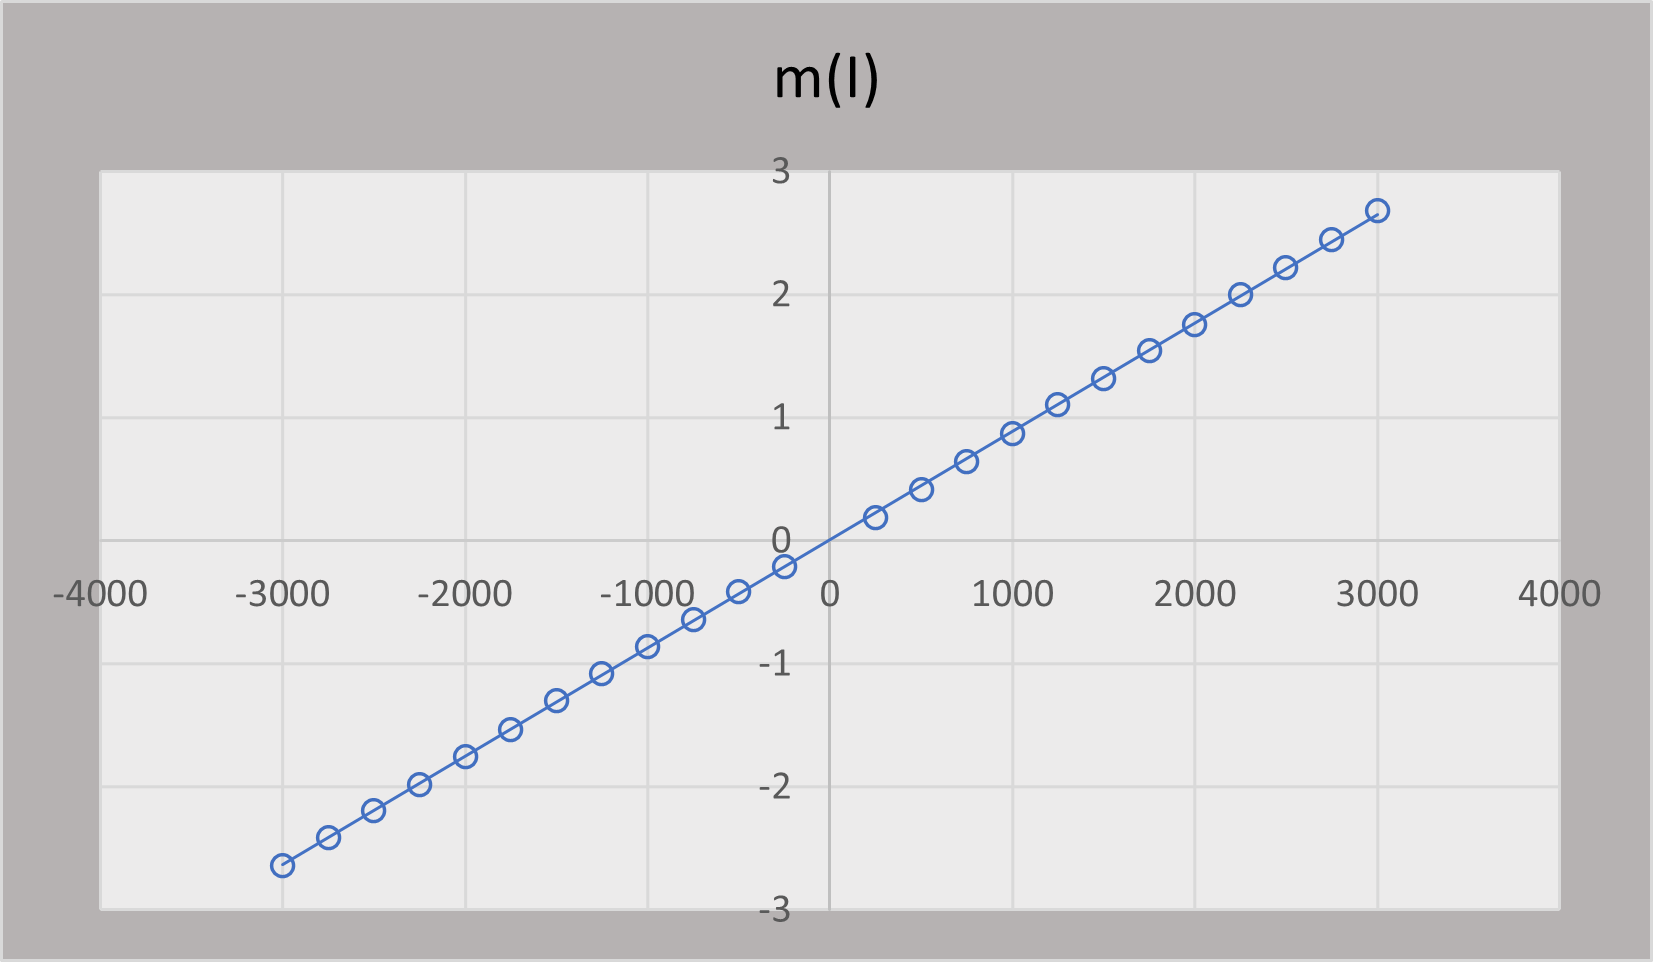
\includegraphics[width=\textwidth]{Graf}
\end{figure}


\end{document}
